\section{Introduction}
\subsection{Motivation}
Robots often have to move in an unknown environment. For that, a robot has to build up a map
and locate itself in this environment. This kind of problem became a large research
field in the last two decades under the name of \textit{Simultaneous Localization and Mapping
(SLAM)}. Most techniques use landmarks seen by a camera. The robot tries
to see the landmarks in two successive images again and estimate its new position by the change
of the landmarks. Figure \ref{fig:grisetti_slam_example} is showing landmarks on the floor prepared 
for the robot so it can use SLAM. But preparation isn't needed every time, higher-priced vacuum cleaning 
robots for example using SLAM with a camera looking at the ceiling.

\begin{figure}[h!]
	\centering
	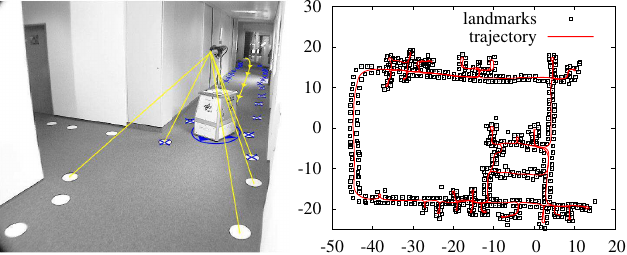
\includegraphics[width=0.5\textwidth]{images/grisetti_slam_example.png}
	\caption{
		An illustration for SLAM with prepared environment for the robot.
		Landmarks are mounted on the floor which the robot can recognize (left image).
		The generated map is shown on the right \cite{grisetti_tutorial_2010}.
		}
	\label{fig:grisetti_slam_example}
\end{figure}

Recent researchers are trying to use physical phenomena instead of landmarks with promising results. 
For example wifi signal or the magnetic field. This opens a completely new variety of possible applications. 
Environments where landmarks of a camera are not suitable for SLAM applications like underwater. Also, scenarios 
where monitoring of a physical phenomenon is the aim and this phenomenon is also suitable for SLAM. So, there
is no need for extra equipment mounted on the robot which saves money.

However, switching from landmarks to physical phenomena is not trivial. The main difference is that landmarks
are discrete in space and physical phenomena are continuous and there can't be made any assumptions to the
underlying function (e.g. it can be described by a polynomial). Moreover, a moving robot will see different
landmarks multiple times and can set its position in relation to it. In case of physical phenomena,
there are only measurements possible at the current position of the robot which is uncertain. But every 
measurements are correlating which can be used to estimate a position or trajectory of the robot. This 
correlation is modeled within the covariance matrix of a gaussian process which will be discussed in 
\ref{chap:gaussian}.